\section{Approach}
\label{sec:approach}
We first give some preliminary definitions, then present our base model.
The high-level overview of our framework is illustrated in \figref{fig:arch}, 
and we next zoom into each of the components to 
present how our framework incorporates implicit positive and negative feedback.

\subsection{Preliminaries}
In the typical session-based setting, given the prefix sequence of the session, denoted as $S_u=(n_1, n_2,...,n_T)$, our goal is 
to predict $n_{T+1}$ article that the target user $u$ is most likely to click next. 
Following~\citeauthor{liu2018stamp}, we use an $N\times d_n$ 
item embedding matrix, where $d_n$ is the embedding dimensionality, to provide article $n_i$'s embedding vector
as $\mathbf{x}_i$. Then methods like RNN~\cite{hidasi2018recurrent}, GNN~\cite{wu2019session,pan2020star}, 
or attention-based approaches~\cite{kang_self-attentive_2018,liu2018stamp} can be used to 
encode the session information into vector $\mathbf{x_s}$ from the sequence 
${(\mathbf{x}_1, \mathbf{x}_2, ..., \mathbf{x}_T)}$, which represents the user's history preferences.
Meanwhile, the same item embedding matrix can be also regarded as $N$ encoded candidates $[\mathbf{x}_1, \mathbf{x}_2,.., \mathbf{x}_N]$.
For $u$, the cosine similarity score $\hat{z_j}^u$ between the session representation and the article $n_j$ is calculated by the inner product of the session vector $\mathbf{x_s}$ and the candidate news article's vector:
\begin{equation}
    \label{eq:zj}
    \hat{z_j}^u = \mathbf{x}_j^T\mathbf{x_s}, j\in[1,N],
\end{equation}
\begin{equation}
    \label{eq:yy}
    \hat{\mathbf{y}}^u = softmax(\hat{\mathbf{z}}^u),
\end{equation}
$\hat{y_j}^u$ is normalized by softmax function in \eqnref{eq:yy} to be the probability of article $j$ being clicked next in the session. 
The cross-entropy is usually used to compute loss:
\begin{equation}
    \mathcal{L}_1 = - \frac{1}{|S|}\sum_{S_u \in S}\sum_{j=1}^N ( y_j^u \log(\hat{y_j}^u) + (1-y_j^u)\log(1-\hat{y_j}^u)),
\end{equation}
where $S$ is the whole training sessions, $y_j^u=1$ if $n_j$ is indeed the next-clicked articles $n_{T+1}$ in $S_u$ and $y_j^u=0$ otherwise.

\begin{figure}[th]
    \centering
    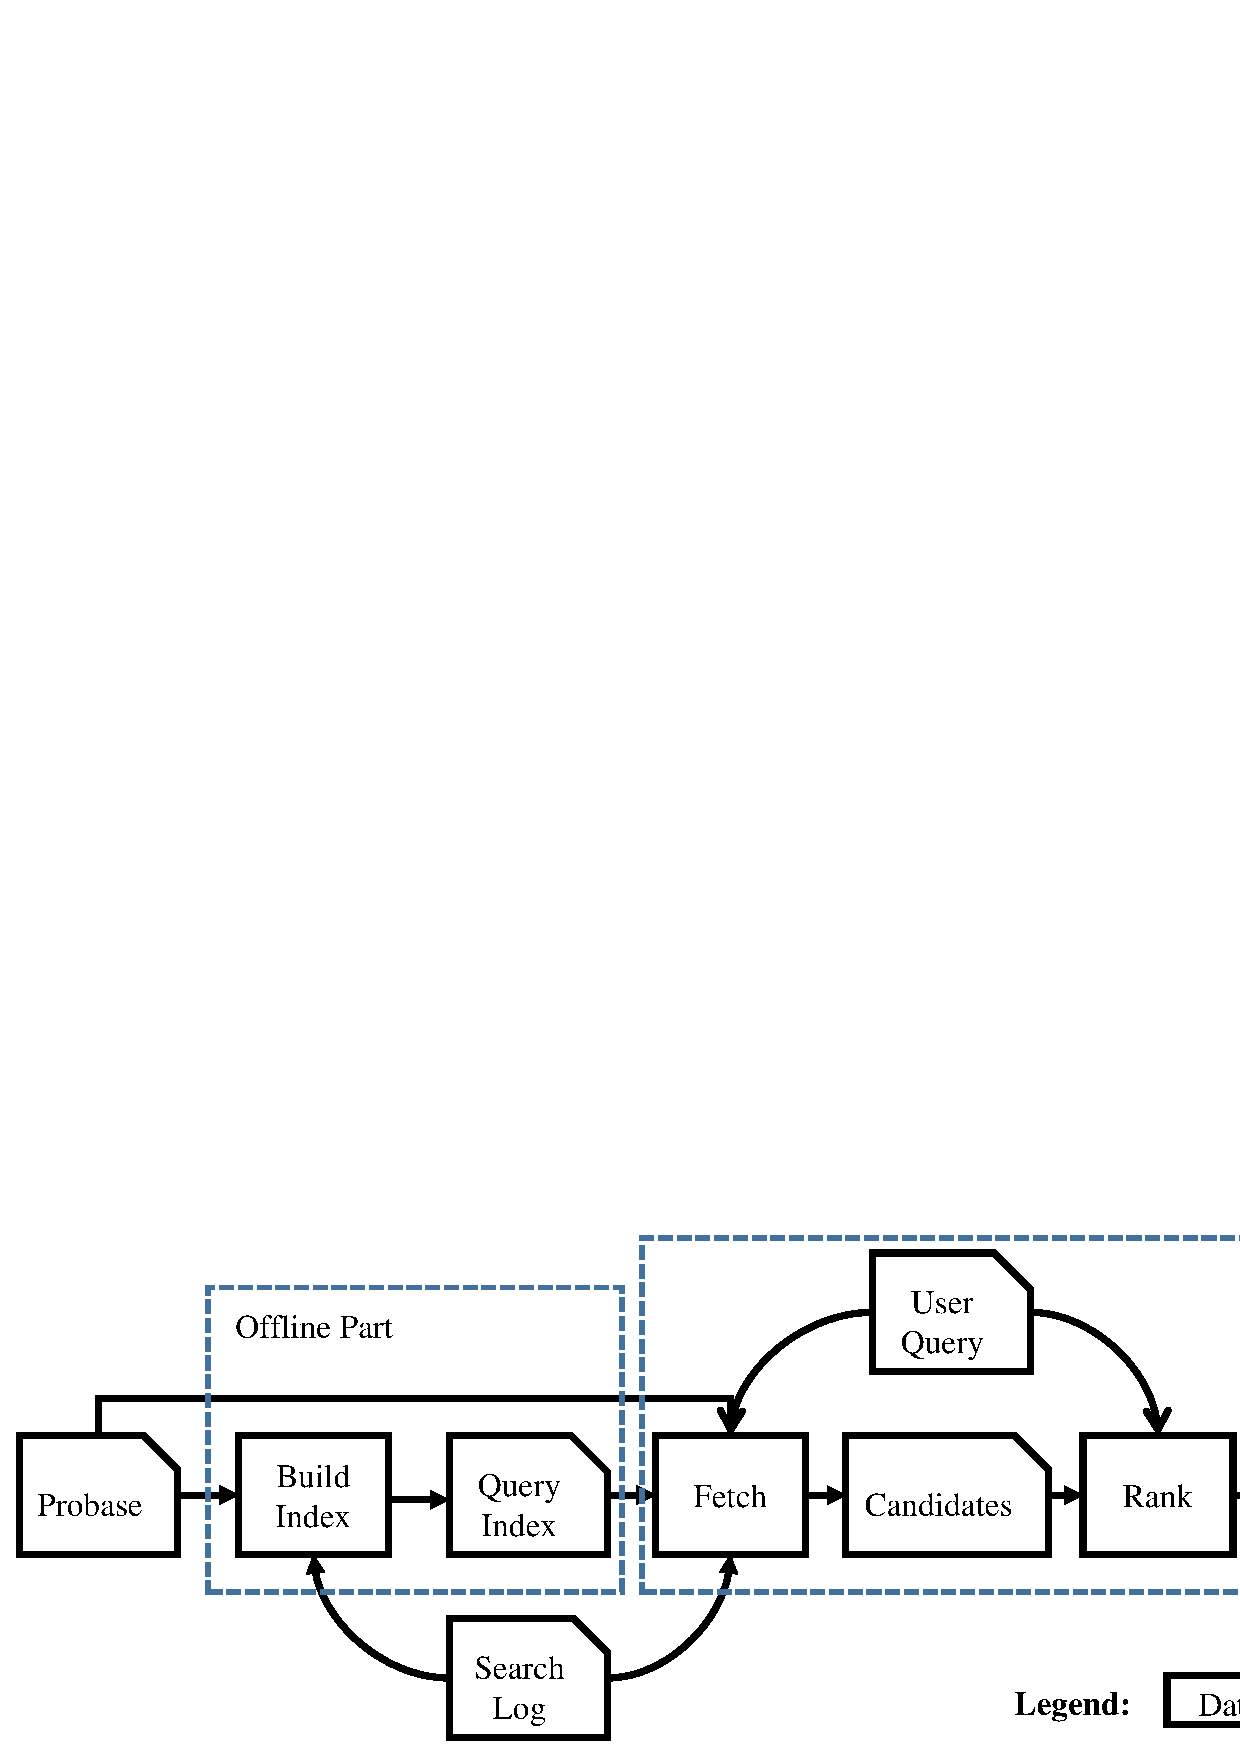
\includegraphics[width=\columnwidth]{fig/architecture.pdf}
    \caption{The architecture of our model.}
    \label{fig:arch}
\end{figure}

\subsection{Content-aware Recommendation (CAR)}
In order to recommend new and emerging articles,
our starting point is a basic content-aware recommendation model. 
To encode articles' content information, 
\citeauthor{moreira2019contextual} uses pre-trained article content embeddings, 
which is supervised trained based on the Word2Vec word embeddings in news titles and the metadata attributes of articles, such as categories.
Specifically, we get the $d_c$-dimensional vectors from Word2Vec to represent the 
topic-oriented content of articles. Once we get the content vector $c_i$ of 
article $n_i$, we concatenate $c_i$ and $\mathbf{x}_i$ to represent 
the article as $\mathbf{x_{c}}_i$. 
To model the varying user preference to the articles in the same session, mainly following~\citeauthor{liu2018stamp}, we adopt a simple attention network, using the weighted sum of the input sequence of vectors to encode the whole session.

We define $\alpha_i$, the attention weight of $i$-th articles $n_i$ in session $S_u$ as:
\begin{equation}
    \label{eq:alpha}
    \alpha_i = W_0 \times \sigma (W_1 \times \mathbf{x_{c}}_i +  b_1),
\end{equation}
\begin{equation}
    \alpha_i^{\prime} = \frac{exp(\alpha_i)}{\sum_{i=1}^T exp(\alpha_i)},
\end{equation}
where $W_0\in \mathbb{R}^{1 \times d_n}, W_1 \in \mathbb{R}^{d_n\times (d_n+d_c)}$ 
are weighting parameters, $\mathbf{x_{c}}_i$ is the article vector, 
and $b_1\in \mathbb{R}^{d_n}$ is a bias. $\alpha_i^{\prime}$ is normalized by softmax.

Finally, $\mathbf{x_s}$ of session $S_u$ is defined as the weighted sum:
\begin{equation}
    \label{eq:final_repre}
    \mathbf{x_s} = \sum_{i=1}^{T} \alpha_i^{\prime} \mathbf{x_{c}}_i.
\end{equation}

At the same time, when computing $\mathcal{L}_1$, the $\mathbf{x}_j$ in \eqnref{eq:zj} should be replaced by $\mathbf{x_{c}}_j$.

\subsection{Utilize Positive Feedback}
\label{sec:positive feedback}
Our implicit positive feedback takes the form of the \textit{active time} interval that 
a user spent on each article after clicking on it. If the user spends a short time 
in an article, it's probably because the user is fooled by the title but actually doesn't like 
the article~\cite{lu_quality_2019}. Note that if the active time is not explicitly available, 
it can be estimated by the time interval between the user's two consecutive clicks. 
For the different and continuous active time $t_i$, 
we bucketize them into a discrete variable~\cite{wu2020CPRS} by: 
\begin{equation}
    t_i^{\prime}=\lfloor log_2{t_i} \rfloor,
\end{equation}
and we map discrete $t_i^{\prime}$ into $m$ distinct categories, 
where each category shares the same embedding vector $\mathbf{ta}_i$, representing the degree  of positive feedback. We feed this vector into the attention computation as extra click-level 
feedback. Now, $\alpha_i$ in \eqnref{eq:alpha} is modified to:
\begin{equation}
    \alpha_i = W_0 \times \sigma (W_1 \times \mathbf{x_{c}}_i + W_2 \times \mathbf{ta}_i + b_1),
\end{equation}
where $W_2 \in \mathbb{R}^{d_n \times d_t}$ is projection parameters that map active time embeddings with $d_t$ dimension into another dimension space. The final session vector $\mathbf{x_s}$ still follows
\eqnref{eq:final_repre}.

\subsection{Joint Learning with Negative Feedback}
\label{sec:negative feedback}
The most straight-forward and widely adopted negative sampling strategy is the random sampling 
from a non-clicked set of items, or from a global buffer with the last $N$ 
clicks~\cite{moreira_news_2018}. 
The major problem of randomly sampled items is that these items might be completely unrelated to 
the user, posing too little challenge for the model to learn. On the contrary, an informative item should be able to confuse the model whether it has discovered more complex hidden meaning of user interaction or not.

While reading news, a user scrolls up and down the news stream, 
and the articles that are exposed to the user collectively 
form an impression list $Imp_u$. We take unclicked articles in $Imp_u$ as more informative negative signals than other candidates~\cite{xie2020deep} and thus wes should treat them differently when counting loss, which means we should penalty the similarity between $\mathbf{x_s}$ and those strong negative samples more strictly. This idea is similar to utilizing grayscale data~\cite{lin2020world} and contrastive learning~\cite{saunshi2019theoretical}, where we both consider the different degrees of information carried from different items.

As we discussed before, since the impression list is not always explicitly available, 
we assume an article is more likely to be in $Imp_u$ if it was published nearby an article that has
been clicked by $u$. Specifically, we keep the nearby articles with the window size 300 and sample items from this window.
We aim to minimize the cosine score between $\mathbf{x_s}$ and the vector $\mathbf{x_{c}}_j$ of negative sample 
$n_j\in Ne_u$, where $Ne_u\subseteq Imp_u$ is the set of negative samples for session $S_u$, thus we add this constraint into the final loss: 

\begin{equation}
    \label{eq:loss}
    \begin{split}
        \mathcal{L}_2 = - \frac{1}{|S|} & \sum_{S_u \in S}\sum_{j=1}^N ( y_j^u \log(\hat{y_j}^u) + (1-y_j^u)\log(1-\hat{y_j}^u) \\
        & +  \lambda \mathbbm{1}(n_j \in Ne_u) \log(\sigma(1-\mathbf{x_{c}}_j^T\mathbf{x_s}))),
    \end{split}
\end{equation}
where $\mathbbm{1}(\cdot)$ returns 1 if the expression is true, $\lambda$ is 
the weighting parameter of loss from negative articles. We jointly optimize these two losses 
with Adam optimizer. 